%Copyright 2014 Jean-Philippe Eisenbarth
%This program is free software: you can 
%redistribute it and/or modify it under the terms of the GNU General Public 
%License as published by the Free Software Foundation, either version 3 of the 
%License, or (at your option) any later version.
%This program is distributed in the hope that it will be useful,but WITHOUT ANY 
%WARRANTY; without even the implied warranty of MERCHANTABILITY or FITNESS FOR A 
%PARTICULAR PURPOSE. See the GNU General Public License for more details.
%You should have received a copy of the GNU General Public License along with 
%this program.  If not, see <http://www.gnu.org/licenses/>.

%Based on the code of Yiannis Lazarides
%http://tex.stackexchange.com/questions/42602/software-requirements-specification-with-latex
%http://tex.stackexchange.com/users/963/yiannis-lazarides
%Also based on the template of Karl E. Wiegers
%http://www.se.rit.edu/~emad/teaching/slides/srs_template_sep14.pdf
%http://karlwiegers.com
\documentclass{scrreprt}
\usepackage{listings}
\usepackage{underscore}
\usepackage{graphicx}
\usepackage[bookmarks=true]{hyperref}
\usepackage[utf8]{inputenc}
\usepackage[romanian]{babel}
\hypersetup{
    bookmarks=false,    % show bookmarks bar?
    pdftitle={Document de specificare a cerințelor software},    % title
    pdfauthor={N. Boca, Ș. Ignătescu, G. Răileanu},                     % author
    pdfsubject={TeX and LaTeX},                        % subject of the document
    pdfkeywords={TeX, LaTeX, graphics, images}, % list of keywords
    colorlinks=true,       % false: boxed links; true: colored links
    linkcolor=blue,       % color of internal links
    citecolor=black,       % color of links to bibliography
    filecolor=black,        % color of file links
    urlcolor=purple,        % color of external links
    linktoc=page            % only page is linked
}%
\def\myversion{1.0 }
\date{}
%\title
\usepackage{hyperref}
\begin{document}

\begin{flushright}
    \rule{16cm}{5pt}\vskip1cm
    \begin{bfseries}
        \Huge{DOCUMENT DE SPECIFICARE A\\CERINȚELOR SOFTWARE}\\
        \vspace{1.7cm}
        pentru\\
        \vspace{1.7cm}
        Proiect - inferența prin enumerare\\
        \vspace{1.7cm}
        \LARGE{Versiunea \myversion}\\
        \vspace{1.7cm}
        Creat de N. Boca, Ș. Ignătescu, G. Răileanu\\
        \vspace{1.7cm}
        Universitatea Tehnică „Gheorghe Asachi” Iași\\
        \vspace{1.7cm}
        \today\\
    \end{bfseries}
\end{flushright}

\tableofcontents
%\chapter*{Revision History}

%\begin{center}
%    \begin{tabular}{|c|c|c|c|}
%        \hline
%	    Name & Date & Reason For Changes & Version\\
%        \hline
%	    21 & 22 & 23 & 24\\
%        \hline
%	    31 & 32 & 33 & 34\\
%        \hline
%    \end{tabular}
%\end{center}

\chapter{Introducere}

\section{Scopul documentului}
Scopul acestui document este descrierea cu exactitate a capabilităților pe care produsul software \textit{Bayesian Network Medical Application} le oferă utilizatorilor săi finali, specificând cerințele funcționale și non-funcționale pe care aplicația le implementează.

\section{Convențiile documentului}
Documentul urmărește formatarea standard IEEE pentru dezvoltarea de software. Standardul definește o formatare obișnuită a documentului care urmează, incluzând scrierea la persoana a III-a, voce pasivă, precum și text coerent și corect din punct de vedere gramatical.

\section{Publicul destinat}
Documentul este destinat publicului tehnic, care deține cunoștințe de bază ale unor limbaje de programare orientate-obiect, alături de noțiuni elementare de statistică, necesare pentru înțelegerea problematicii expuse.

\section{Scopul produsului}
\textit{Bayesian Network Medical Application} este o aplicație dezvoltată în limbajul C\#. Cu ajutorul aplicației se poate determina probabilitatea existenței unei anumite afecțiuni cunoscând simptomele pe care aceasta le manifestă.

\section{Referințe}
Programul descris a avut ca referință aplicația din laboratorul numărul 11 cu tema „Rețele bayesiene” a cursului de Inteligență Artificială (prof. Florin Leon, Facultatea de Automatică și Calculatoare din Iași). De asemenea, implementarea are la bază limbajul C\#, dezvoltat de Microsoft.

\chapter{Descrierea generală}

\section{Perspectivele produsului}
Deși există numeroase sisteme expert sau motoare de inferență care pot calcula probabilități dându-se date cunoscute, aplicația de față se folosește în calcul de metoda inferenței prin enumerare, caracteristică rețelelor bayesiene. Faptul că astfel de rețele sunt deseori reprezentate prin intermediul grafurilor ajută în procesul de înțelegere, acest lucru constituind un avantaj față de celelalte metode expuse.\par
\textbf{Adaugă aici o poză cu interfața (sau cu componente: dll-ul și modulul din care îl apelăm)}

\section{Funcțiile produsului}
\begin{itemize}
	\item generare noduri personalizate și relații de precedență: utilizatorul poate determina propria rețea bayesiană de lucru
	\item încărcarea valorilor probabilistice din interfață sau dintr-o sursă externă
	\item calcul de probabilități folosind noduri observate și noduri evidență
\end{itemize}

\section{Clase de utilizatori și caracteristici}
Întrucât aplicația este una de uz general, nu există o categorie de utilizatori aparte. Ea este accesibilă oricui și poate fi folosită.

\section{Mediul de utilizare}
Pentru executarea aplicației este nevoie de un sistem de operare Windows. Alternativ, pentru utilizatorii sistemelor UNIX/Linux se pot pot folosi soluții precum \textit{Wine} sau \textit{Mono}, care permit rularea aplicației.

\section{Proiectarea și implementarea constrângerilor}
Aplicația dispune de o licențiere MIT, dezvoltatorul fiind responsabil pentru orice extindere a funcționalităților aplicației. Aceasta poate interfața cu alte limbaje de programare și poate expune.\par
\textbf{Aici, facem MVP???}

\section{Documentația utilizatorului}
Utilizatorul poate folosi ghidul aplicației, pus la dispoziție de către dezvoltatori în format \textbf{.chm}.

\section{Ipoteze și dependențe}
$<$List any assumed factors (as opposed to known facts) that could affect the 
requirements stated in the SRS. These could include third-party or commercial 
components that you plan to use, issues around the development or operating 
environment, or constraints. The project could be affected if these assumptions 
are incorrect, are not shared, or change. Also identify any dependencies the 
project has on external factors, such as software components that you intend to 
reuse from another project, unless they are already documented elsewhere (for 
example, in the vision and scope document or the project plan).$>$


\chapter{Cerințe externe de interfață}

\section{Interfața cu utilizatorul}
Pentru introducerea ușoară a datelor de intrare și pentru a vedea rezultatul final, aplicația dispune de o interfață grafică, prezentată în figura de mai jos:

\begin{center}
	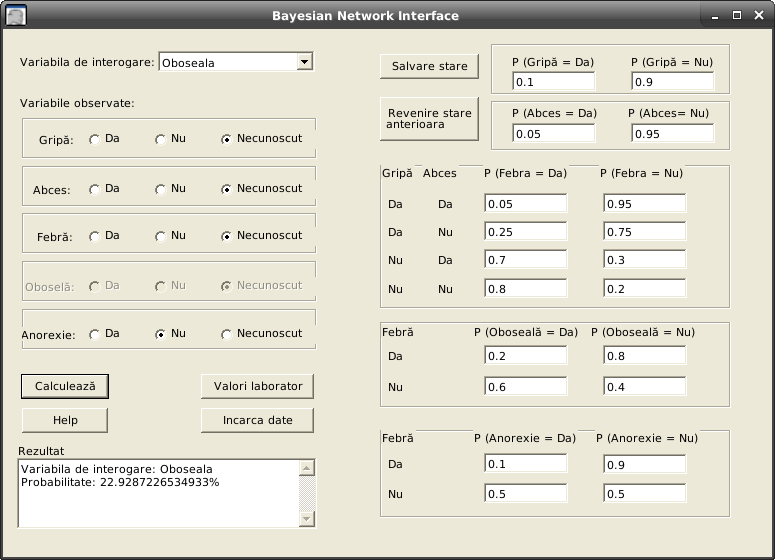
\includegraphics [scale=0.5] {img/gui.png}
\end{center}

Această interfață pune la dispoziția utilizatorului posibilitatea de a selecta variabila de interogare dintr-o listă de simptome și variabilele de evidență împreună cu datele cunoscute despre apariția acestora.

Probabilitățile de apariție ale simptomelor pot fi introduse atât manual prin câmpurile de text marcate, cât și încărcate din fișiere externe. După apăsarea butonului \textit{Calculează}, programul analizează toate datele primite și afișează rezultatul în câmpul de text din stânga jos.

Programul pune la dispoziție valorile probabilităților utilizate în laborator, iar la apăsarea butonului \textit{Valori laborator} acestea vor popula câmpurile de text. Pentru a importa date din alte fișiere externe, acestea trebuie să aibă denumirea de forma \textit{simptom.txt} și să conțină lista de probabilități ale cazurilor de adevăr. Fișierele în formatul specificat anterior vor fi salvate in folderul \textit{probabilities/date} din cadrul soluției, iar datele vor fi încărcate în program la apăsarea butonului \textit{Încarcă date}.

În cazul introducerii valorilor de probabilitate în mod manual, utilizatorul va fi împiedicat să scrie date eronate, iar câmpurile alăturate se vor completa automat pentru a ușura acest proces.


\section{Interfața hardware}
Fiind un produs software, acesta nu dispune de o interfață hardware dedicată.

\section{Interfața software}
Aplicația de față nu necesită o conexiune cu baza de date, toate datele necesare fiind cele inițiale. Acestea sunt stocate în fișiere, neexistând o justificare pentru a folosi o bază de date. Nu există o comunicare a aplicației cu alte componente ale sistemului de operare/elemente hardware.

\section{Interfața de comunicare}
Aplicația este livrată ca software independent și nu necesită alte componente pentru comunicare, fiind gândită să fie \textit{self-contained}.

\chapter{Cerințe funcționale}
\textbf{?? Vezi exact ce se întâmplă aici}

\section{Cerințe de performanță}
Aplicația va oferi răspunsul cerut de utilizator în timp real și o aproximare cât mai exactă, aceasta depinzând de precizia calculatorului pe care este rulată.

\subsection{Cerințe de fiabilitate}
Întrucât aplicația este una software, fiabilitatea ei este determinată de cerințele sistemului pe care rulează. Astfel, pot apărea erori la migrarea aplicației pe o altă platformă cu o configurație diferită, deși acest lucru este puțin probabil în cazul migrării către configurații cu aceeași familie de sisteme de operare.

\subsection{Cerințe de securitate}
Sistemul nu necesită măsuri de securitate, altele în afara de cele recomandate pentru sistemul dumneavoastră de operare, neavând acces la componente esențiale din nucleul sistemului de operare și nici la alte fișiere din sistem.

\section{Appendix A: Glossary}
?? Need this?

\end{document}
